\section{PSP Setup}

\subsection{Schematic Diagram}
A generalized schematic setup of phase-shift profilometry is shown in Figure \ref{fig:setup}. It consists of a projector for projecting the fringes and a camera for recording. $p(x,y)$ is an arbitrary point in the object surface with a corresponding value in the image.

\captionsetup[figure]{width=5in}
\begin{figure}[h!]
	\centering
	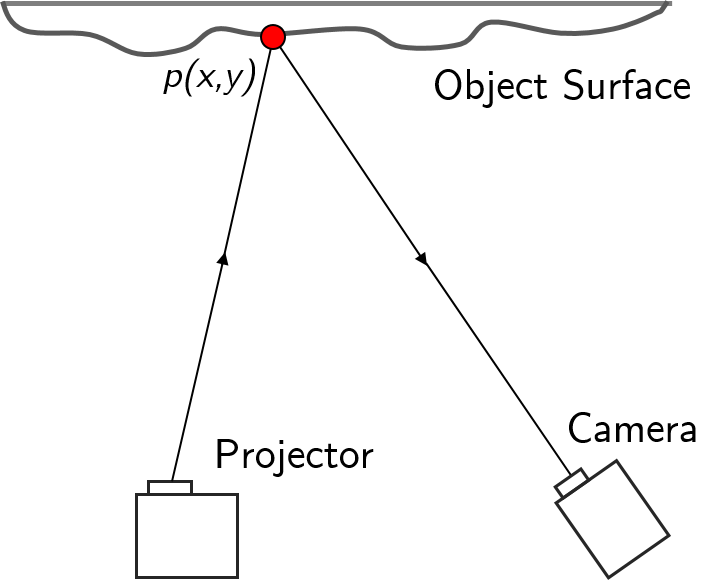
\includegraphics[width=0.475\textwidth]{figures/schematic2.jpg}
	\caption[Simplified schematic diagram of the PSP setup]{Simplified schematic diagram of the PSP setup.}
	\label{fig:setup}
\end{figure}


\subsection{Actual Setup}

An Acer DLP Projector with a resolution of 858 x 600 pixels was used to project the sinusoidal fringes to the target object and the reference in the form of a flat white board. The projected fringes were recorded by an Olympus E-500 8-megapixel DSLR Camera. 

An exposure time of 2.5 seconds for a camera aperture of f/22 was used most of the time for the camera settings. This relatively long exposure time for capturing can already be considered as ``averaging'' for reduction of noise. Images were saved as TIFF files with 3264 x 2448 pixel resolution. 

\captionsetup[figure]{width=5in}
\begin{figure}[h!]
	\centering
	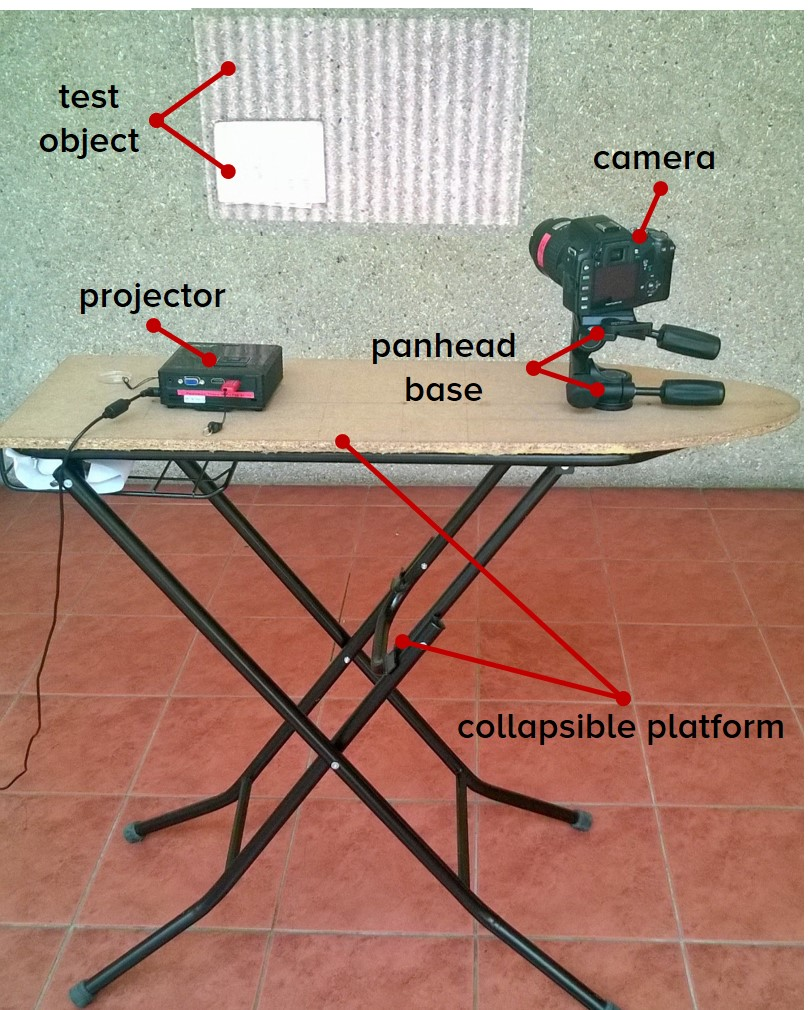
\includegraphics[width=0.42\textwidth]{figures/actualsetup.jpg}
	\caption[Actual PSP setup]{PSP experimental setup.}
	\label{fig:actual}
\end{figure}

In PSP, the stability of the setup is crucial to the output 3D reconstruction as system vibration while projecting the fringes may produce an inappropriate shift leading to error in phase computation. 

A portable mobile set-up was designed for easy-use on \textit{in-situ} experiments without sacrificing stability. The projector and camera are contained on a collapsible platform  which can be easily assembled. The camera is mounted on a panhead base for easy rotation and tilting while still maintaining its alignment with the projector. The projector is screwed on the platform to ensure that no movements will occur during fringe projection.
Shown in Figure \ref{fig:actual} is the actual setup used for PSP acquisition.
